\documentclass[11pt]{article}
\usepackage{hyperref}
\usepackage{amssymb}
\usepackage{amsmath}
\usepackage{epsfig, graphics, graphicx}
\usepackage{latexsym}
\usepackage{fullpage}
\usepackage[parfill]{parskip}
%\usepackage{mysymbols}
\usepackage[tight]{subfigure}
\usepackage{hyperref}
\usepackage{amsmath,amssymb,enumerate,comment}

% reset footnote numbers on each page
\usepackage{perpage}
\MakePerPage{footnote}

\newcommand{\figref}[1]{Fig.~\ref{#1}}
\newcommand{\qed}{\quad \ensuremath{\blacksquare}}      % QED square
\newcommand{\inv}{^{-1}}                                % inverse operator
\newcommand{\sminus}{\backslash}                        % set minus
\newcommand{\N}{\mathbb{N}}                             % natural numbers
\newcommand{\Z}{\mathbb{Z}}                             % integers
\newcommand{\Q}{\mathbb{Q}}                             % rational numbers
\newcommand{\R}{\mathbb{R}}                             % real numbers
\newcommand{\halpha}{\hat{\alpha}}                      % alpha-hat
\newcommand{\hy}{\hat{y}}                               % alpha-hat
\newcommand{\argmin}{\operatornamewithlimits{argmin}}   % argmin
\newcommand{\argmax}{\operatornamewithlimits{argmax}}   % argmax
\newcommand{\e}{\varepsilon}                            % \varepsilon

\title{10-725 Convex Optimization\\Homework 1}
\author{Shashank Singh\footnote{sss1@andrew.cmu.edu}}
\date{Due September 19, 2013}

\begin{document}

\maketitle

%%%%%%%%%%%%%%%%%%%%%%%%%%%%%%%%%%%%%%%%%%%%%%%%%%%%%%%%%%%%%%%%%
%%%%%%%%%%%%%%%%%%%%%%%%%%%%%%%%%%%%%%%%%%%%%%%%%%%%%%%%%%%%%%%%%
\newpage
\section{Mastery set [25 points] (Aaditya)}
\paragraph{A1 [2]}
$\forall k \in {1,\ldots,n}$, define $S_k := \sum_{i = 1}^k \theta_i$ and
$\displaystyle y_k :=
 \sum_{i = 1}^k \frac{\theta_ix_i}{S_k} \in C$. Suppose
that, for some $k \in {1,\ldots,n-1}$, $y_k \in C$. Then,
\begin{align*}
y_{k + 1}
 & := \sum_{i = 1}^{k + 1} \frac{\theta_ix_i}{S_{k + 1}}
   = \frac{\theta_{k + 1}x_{k + 1}}{S_{k + 1}}
   + \sum_{i = 1}^k \frac{\theta_ix_i}{S_{k + 1}}
   = \frac{\theta_{k + 1}x_{k + 1}}{S_{k + 1}}
   + \frac{S_k}{S_{k + 1}}
     \sum_{i = 1}^k \frac{\theta_ix_i}{S_k} \\
 & = \frac{\theta_{k + 1}x_{k + 1}}{S_{k + 1}}
   + \left( 1 - \frac{\theta_{k + 1}}{S_{k + 1}} \right)
     \sum_{i = 1}^k \frac{\theta_ix_i}{S_k}
   \in C,
\end{align*}
since $C$ is convex. Since $y_1 = x_1 \in C$, by induction on $k$,
$y = y_n \in C$. \qed

\paragraph{A2 [3]}
We showed in class that $conv_2(M)$ is convex. Since each point in $M$ is a
convex combination of points in $M$, $M \subseteq conv_2(M)$, so
$conv_1(M) \subseteq conv_2(M)$. If $C \supseteq M$ is convex, then, by part
A1, any convex combination of points in $M$ is in $C$. Thus,
$conv_2(M) \subseteq conv_1(M)$. \qed

\paragraph{B1 [2+2]}
$HP(a,b)$ is convex. If $\theta \in [0,1]$ and $x_1,x_2 \in HP(a,b)$, then
\[a^T (\theta x_1 + (1 - \theta)x_2)
 = \theta a^Tx_1 + (1 - \theta)a^Tx_2
 = \theta b + (1 - \theta)b
 = b. \qed
\]
If $x_1 \in HP(a,b_1)$ and $x_2 \in HP(a,b_2)$, then, by Cauchy-Schwarz,
\[\|x_1 - x_2\| \geq \left| \frac{a}{\|a\|}(x_1 - x_2) \right|
    = \mbox{\fbox{$\displaystyle \frac{|b_1 - b_2|}{\|a\|}$,}}\]
and it is easily checked that $x_1 = \frac{b_1}{\|a\|^2}a$ and
$x_2 = \frac{b_2}{\|a\|^2}a$ achieve this bound.

\paragraph{B2 [2+2]}
$HS(a,b)$ is convex. If $\theta \in [0,1]$ and $x_1,x_2 \in HS(a,b)$, then
\[a^T (\theta x_1 + (1 - \theta)x_2)
 = \theta a^Tx_1 + (1 - \theta)a^Tx_2
 \leq \theta b + (1 - \theta)b
 = b. \qed
\]
$HS(a_1,b_1) \subseteq HS(a_2,b_2)$ if and only if
$\exists c \in \R$ with $a_1 = ca_2$ and $b_1 \leq cb_2$.

\paragraph{B3 [2]} $\forall x \in \R^d$,
\vspace{-5mm}
\begin{align*}
                & \|u - x\|_2^2 \leq \|v - x\|_2^2 \\
\Leftrightarrow & \|u\|_2 - 2u^Tx + \|x\|_2 \leq \|v\|_2 - 2v^Tx + \|x\|_2 \\
\Leftrightarrow & \|u\| - \|v\| \leq 2(u - v)^Tx.
\end{align*}
Thus, $\{x \in \R^d \, | \, \|u - x\| \leq \|v - x\|\}
 = HS(2(u - v), \|u\| - \|v\|)$, and is thus convex. \qed

\paragraph{C [2+3]}
$\forall \theta \in [0,1], x,y \in \R_+$,
\[f(s(\theta x + (1 - \theta)y)
 = f(\theta sx + (1 - \theta)sy)
 \leq \theta f(sx) + (1 - \theta)f(sy). \qed
\]
Note that, via the change of variables $u = t/x$,
\[F(x)
 = \frac1x \int_0^x f(t) \, dt
 = \frac1x \int_0^1 f(xu) x \, du
 = \int_0^1 f(xu) \, du.
\]
Thus, $\forall \theta \in [0,1], x,y \in \R_+$, by convexity of the function
$u \mapsto f(xu)$,
\begin{align*}
F(\theta x + (1 - \theta)y)
 & = \int_0^1  f((\theta x + (1 - \theta)y)u) \, du \\
 & \leq \int_0^1  \theta f(xu) + (1 - \theta)f(yu) \, du
   = \theta F(x) + (1 - \theta) F(y). \qed
\end{align*}

\paragraph{D [3+2]}
The LP can be written in standard form as an LP over $6$ variables:
\[0 \leq u =
\begin{bmatrix}
x_2 \\
y_2 \\
z_1 \\
z_2 \\
s_1 \\
s_2
\end{bmatrix}, \quad
c =
\begin{bmatrix}
3  \\
-1 \\
1  \\
-1 \\
0  \\
0
\end{bmatrix}
A =
\begin{bmatrix}
1 & 0 & 0 & 0  & 1 & 0 \\
0 & 1 & 0 & 0  & 0 & 1 \\
1 & 1 & 1 & -1 & 0 & 0  \\
\end{bmatrix}, \quad
b =
\begin{bmatrix}
2 \\
2 \\
-1
\end{bmatrix}
\]


The optimum occurs at \fbox{$(x,y,z) = (1,-1,1)$,} when
\fbox{$3x - y + z = 5$.}

\newpage
Shashank Singh\footnote{sss1@andrew.cmu.edu}
\section{LPs and gradient descent in Stats/ML [25 points] (Sashank)}
%TODO
\paragraph{A [4+4+5]}
\begin{enumerate}[(a)]
\item Suppose $\beta$ optimizes (1). Define
\[\beta^+_i
    := \left\{
        \begin{array}{cc}
            \beta_i : & \beta_i \geq 0  \\
            0 : & \mbox{else}
        \end{array}
       \right.,
\]
$\beta^- := \beta^+ - \beta$. Then, $y = X\beta = X(\beta^+ - \beta^-)$
and $\beta^+,\beta^- \geq 0$, so $(\beta^+,\beta^-)$ is feasible for (2). Since
$1^T(\beta^+ + \beta^-) = \sum_{i = 1}^p |\beta_i| = \|\beta\|_1$, the optimum
for (2) is at most $\|\beta_1\|$. \qed

\item Suppose $(\beta^+,\beta^-)$ optimizes (2). Define
$\beta := \beta^+ - \beta^-$. Then, $y = X(\beta^+ - \beta^-) = X\beta$, so
$\beta$ is feasible for (1). Since
$\|\beta\|_1 = \sum_{i = 1}^p |\beta_i| = 1^T(\beta^+ + \beta^-)$, the optimum
for (1) is at most, and therefore equal to, the optimum for (1). \qed

%TODO
\item
\end{enumerate}

\paragraph{B [6+6]}
\begin{enumerate}[(a)]
\item Rewriting in vector notation (where $h_j(x) = x_j \in \R^n$ is the
$j^{th}$ feature vector), we have
\[\halpha_j
    = \argmin_{\alpha_j \in \R} \|\alpha_jh_j(x) + \hy - y\|_2^2
    = \argmin_{\alpha_j \in \R} \|\alpha_jx_j + \hy - y\|_2^2
    = \argmin_{\alpha_j \in \R} \|\alpha_jx_j - (y - \hy)\|_2^2,
\]
from which it is apparent that $\halpha_j$ is the length of the projection of
$y - \hy$ onto $x_j$,
\begin{equation}
\label{eq:halphaj}
\halpha_j
    = \left\langle \frac{x_j}{\|x_j\|}, y - \hy \right\rangle
    = \mbox{\fbox{$\langle x_j, y - \hy \rangle$.}}
\end{equation}
Note that, rewriting terms as vectors, $g$ is a gradient of the $2$-norm
recentered at $y$:
\[g
    = \frac{\partial L(y,\hy)}{\partial \hy}
    = \frac{\partial \|y - \hy\|_2^2}{\partial \hy}
    = 2(\hy - y).
\]
Thus, rewriting again in vector notation, we have
\[
j = \argmin_{\ell \in \{1,\dots,M\}}\|-g - \halpha_\ell h_\ell(x) \|_2^2
  = \argmin_{\ell \in \{1,\dots,M\}}\|\halpha_\ell x_\ell - (y - \hy)\|_2^2.
\]
From (\ref{eq:halphaj}), it is clear that this term is just the error of
approximating $(y - \hy)$ by its projection onto $x_j$. This error is minimized
by maximizing the inner product of $x_j$ and $y - \hy$, and hence
\begin{equation}
\label{eq:jvalue}
 \mbox{\fbox{$\displaystyle
    j = \argmax_{\ell \in \{1,\dots,M\}} |\langle x_j, y - \hy \rangle|.
 $}}
\end{equation}
We could make this derivation a bit more rigorous (find roots of the derivative
to compute $\halpha_j$, and then obtain (\ref{eq:jvalue}) via some algebra),
but these arguments give much better intuition.

\item
\[\halpha_j
    = \argmin_{\alpha_j \in \R} \sum_{i = 1}^n
        \log \left( 1 + \exp(-2y_i(\hy_i + \alpha_jh_j(x_i))) \right).
\]
I don't see a good way of minimizing this analytically. A simple way to
approximately minimize this in practice would be to find the $\alpha_j$ values
that minimize each term of the sum, and then try values of $\alpha_j$ (perhaps
uniformly) in the interval surrounded by those values.
\end{enumerate}

\newpage
Shashank Singh\footnote{sss1@andrew.cmu.edu}
%TODO
\section{Programming gradient descent [25 points] (Yifei)}
\begin{enumerate}[(a)]
\item (5 pts) Based on the plots, $f_Q$, $f_{LL}$, and $f_R$ appear convex,
whereas $f_H$ appears to have minima that are local but not global.
\begin{figure}[h!]
\begin{center}
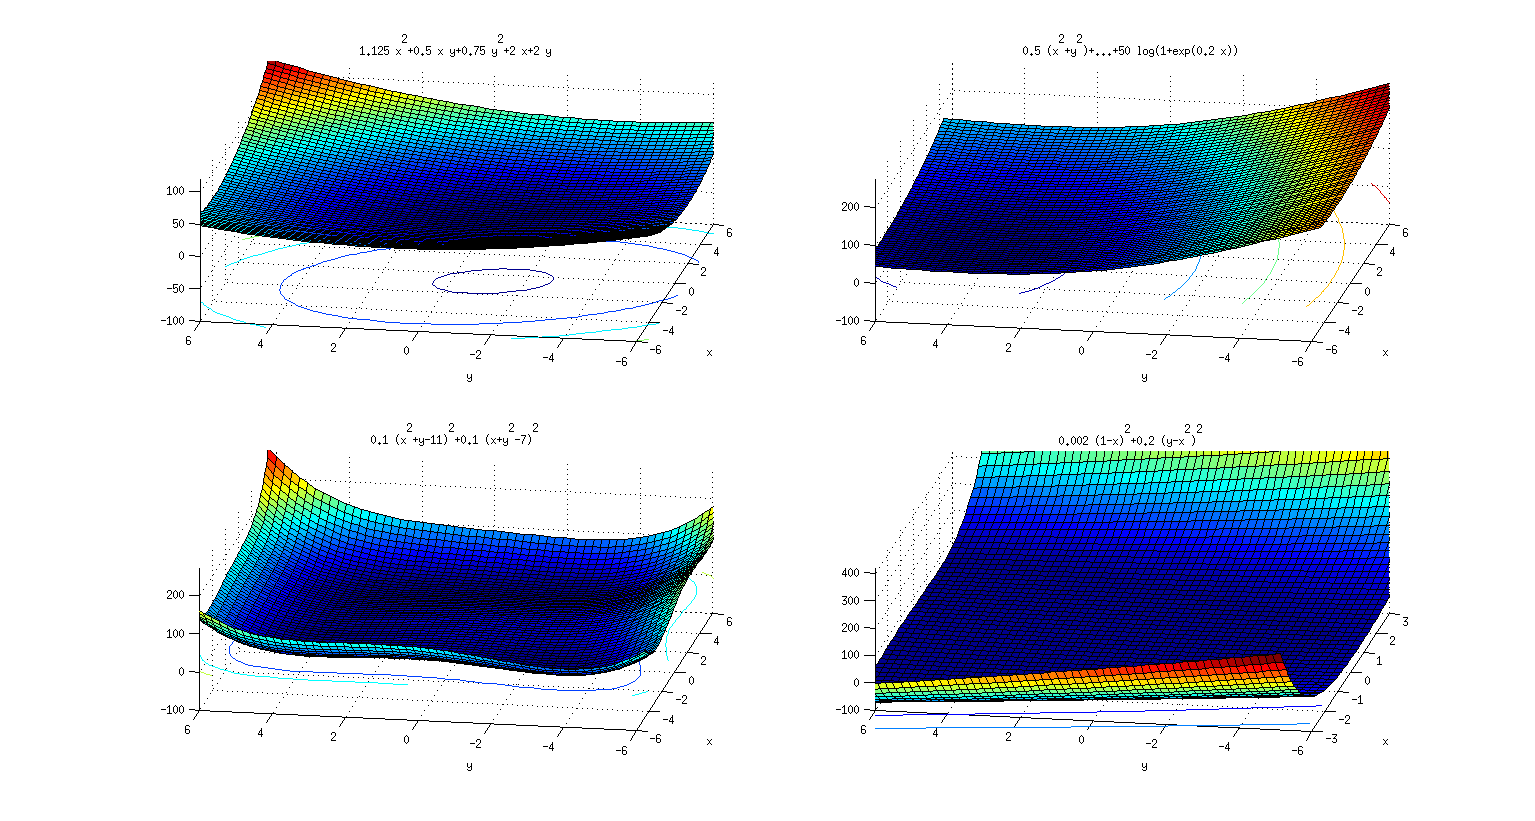
\includegraphics[width=400pt,height=300pt]{fig3a}
\end{center}
\caption{Surface and contour plots of the four objective functions.}
\label{fig:ezsurfc}
\end{figure}
\item (8 pts) In each figure below, the row indicates the step size ($0.3$ or
$0.8$) and the column indicates the initialization ($(2,3)^T$ or random).
\begin{figure}[h!]
\begin{center}
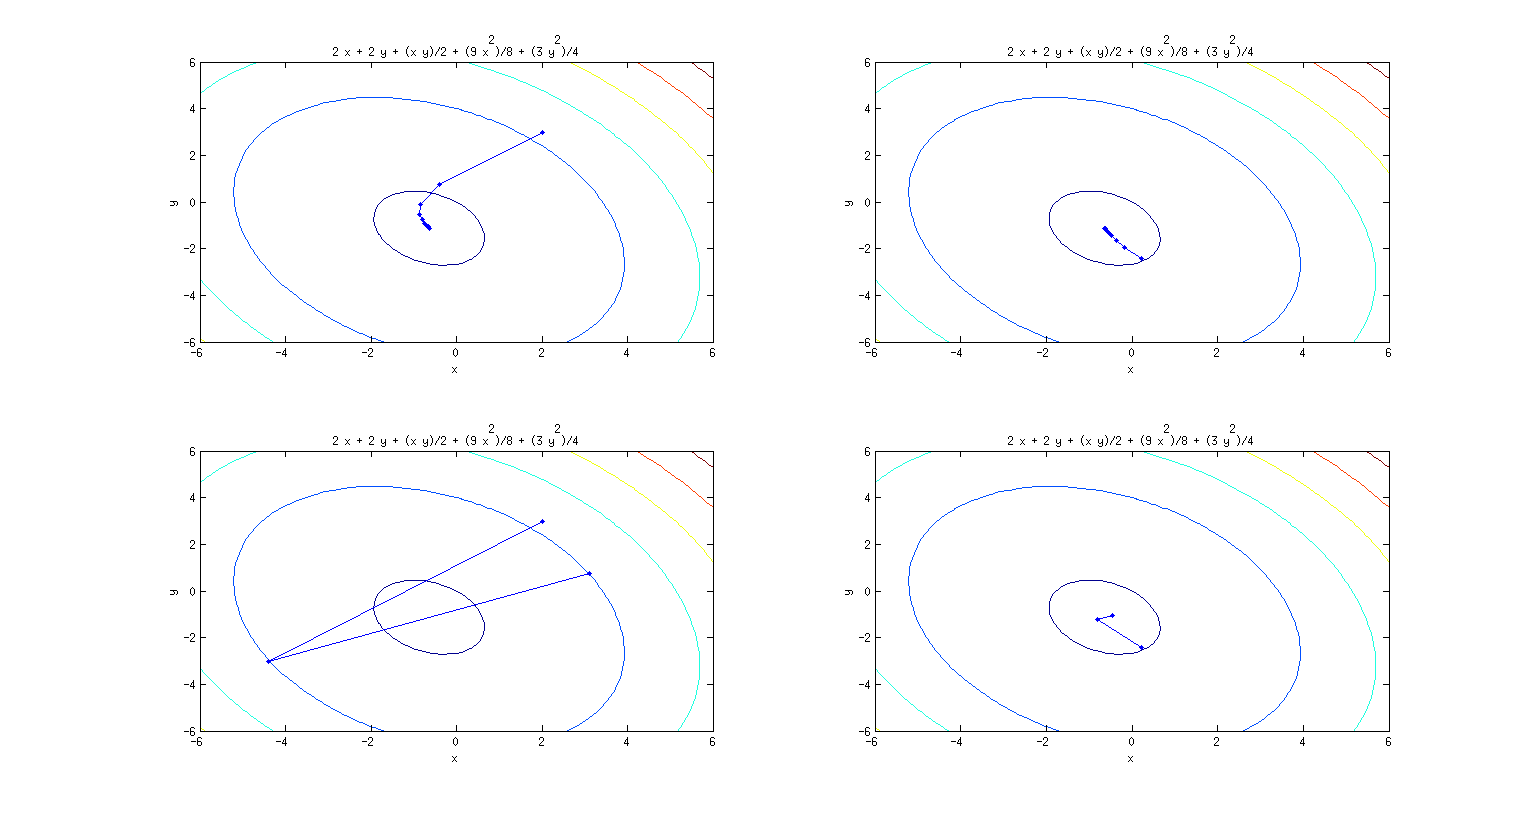
\includegraphics[width=300pt,height=200pt]{fig3b1}
\end{center}
\caption{Gradient descent path and contour plots of $f_Q$ at each step size and
initialization.}
\label{fig:grad1}
\end{figure}
\begin{figure}[h!]
\begin{center}
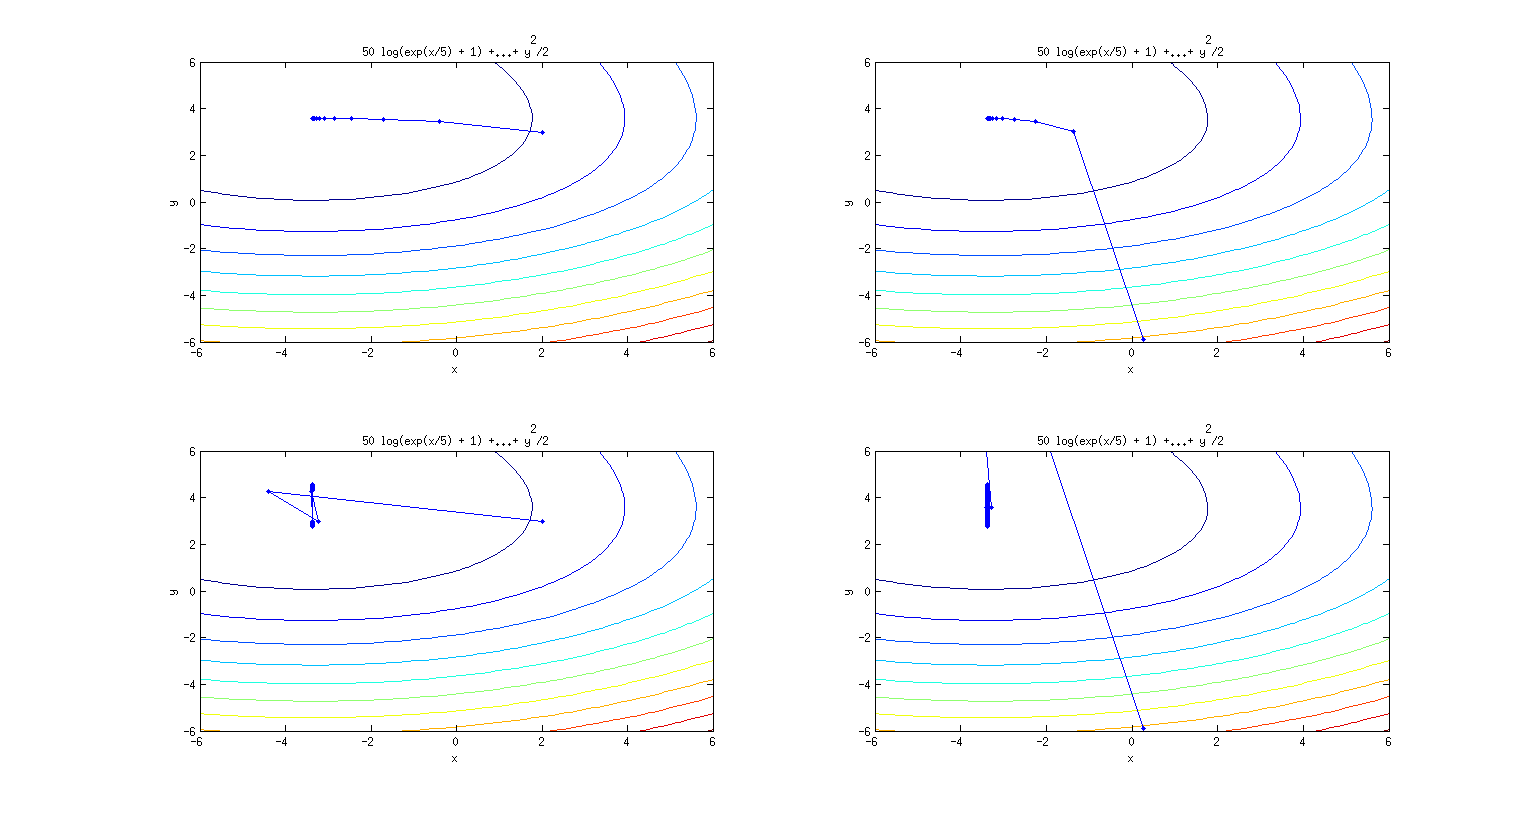
\includegraphics[width=300pt,height=200pt]{fig3b2}
\end{center}
\caption{Gradient descent path and contour plots of $f_{LL}$ at each step size
and initialization.}
\label{fig:grad2}
\end{figure}
\begin{figure}[h!]
\begin{center}
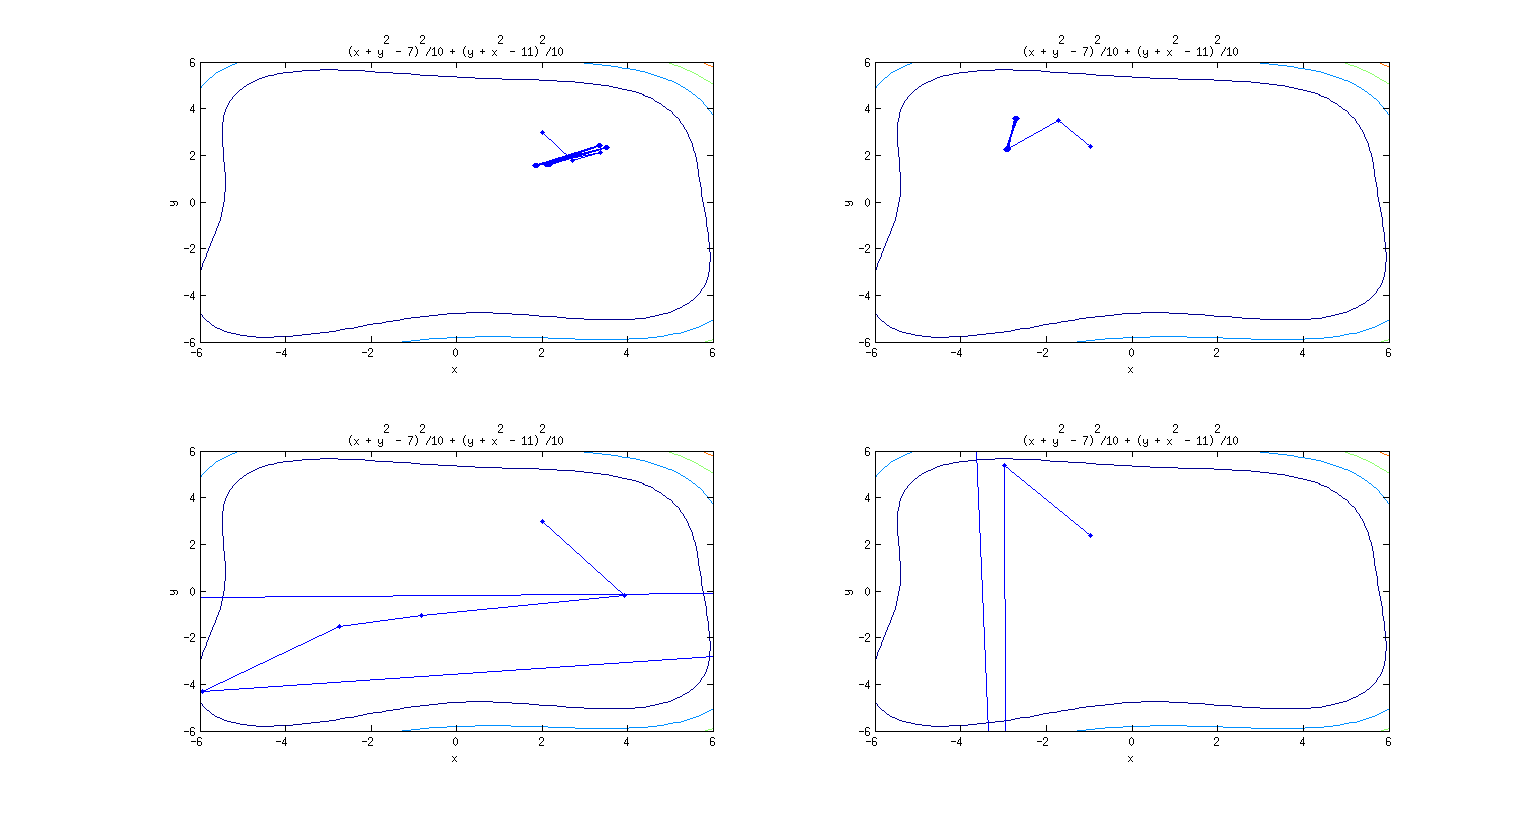
\includegraphics[width=300pt,height=200pt]{fig3b3}
\end{center}
\caption{Gradient descent path and contour plots of $f_H$ at each step size and
initialization.}
\label{fig:grad3}
\end{figure}
\begin{figure}[h!]
\begin{center}
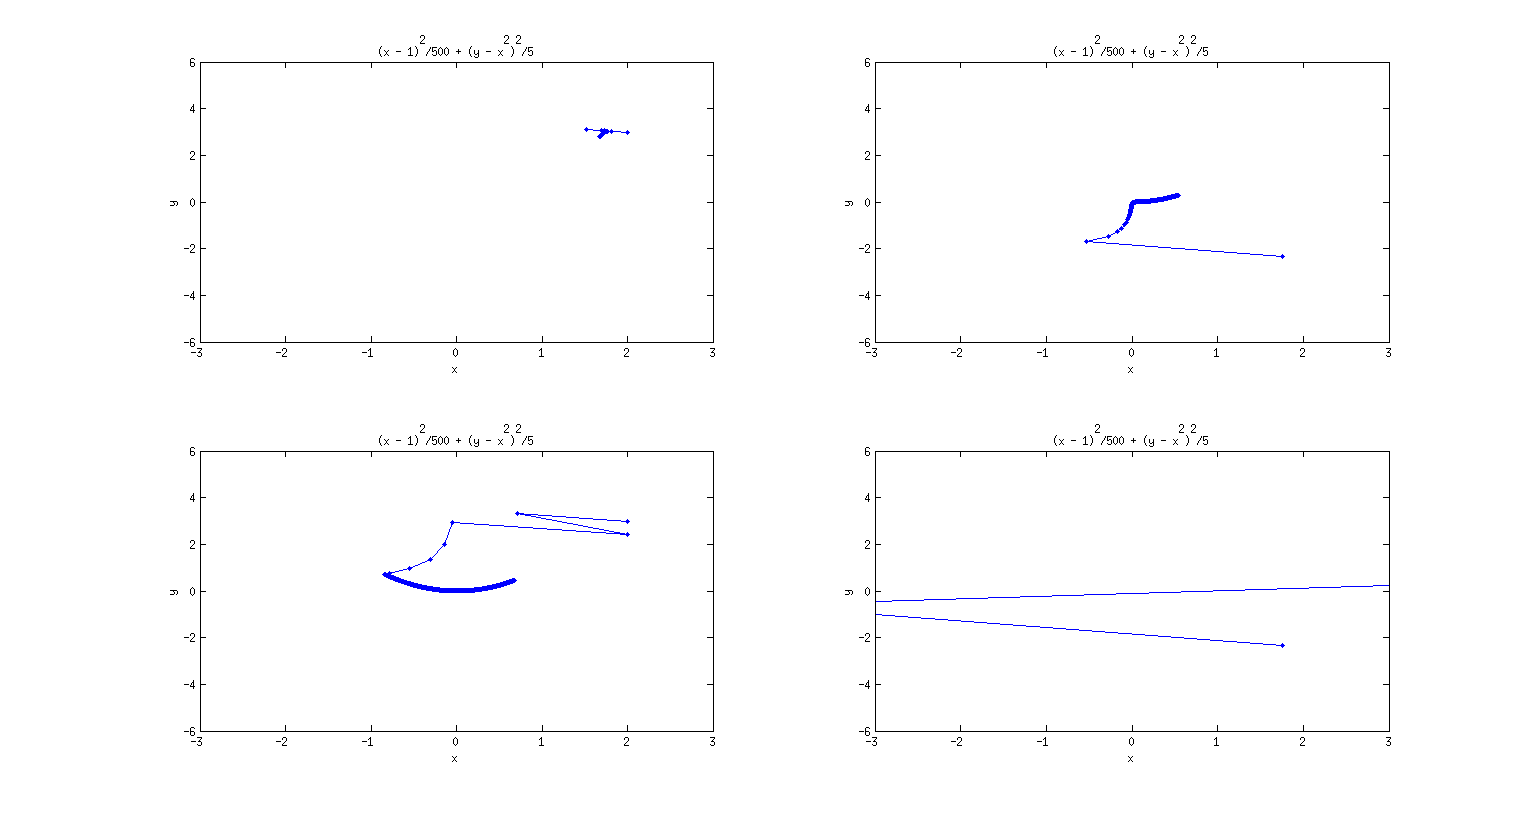
\includegraphics[width=300pt,height=200pt]{fig3b4}
\end{center}
\caption{Gradient descent path and contour plots of $f_R$ at each step size and
initialization.}
\label{fig:grad4}
\end{figure}
%TODO
\item (6 pts)
%TODO
\item (4 pts)
%TODO
\item (2 pts)
\end{enumerate}

\newpage
\null
\newpage
\null
\newpage
Shashank Singh\footnote{sss1@andrew.cmu.edu}
\section{Convergence rate of subgradient method [25 points] (Adona)}
\begin{enumerate}[(a)]
\item (4 pts) Since the $2$-norm is induced by an inner product
$\langle\cdot,\cdot\rangle$,
\begin{align*}
\|x^{(k)} - x^\star\|_2^2
 & = \|x^{(k - 1)} - x^\star - t_kg^{(k - 1)}\|_2^2
                                    & \mbox{(def. of $x^{(k)}$)} \\
 & = \langle x^{(k - 1)} - x^\star - t_kg^{(k - 1)},
             x^{(k - 1)} - x^\star - t_kg^{(k - 1)} \rangle \\
 & = \|x^{(k - 1)} - x^\star\|_2^2
   - 2t_k \langle x^{(k - 1)} - x^\star,g^{(k - 1)}\rangle
   + t_k^2\|g^{(k - 1)}\|_2^2
                    & \mbox{(bilinearity of $\langle\cdot,\cdot\rangle$)} \\
 & \leq \|x^{(k - 1)} - x^\star\|_2^2
   - 2t_k \left(f(x^{(k - 1)}) - f(x^\star)\right)
   + t_k^2\|g^{(k - 1)}\|_2^2,
\end{align*}
where the inequality follows from the definition of a subgradient. \qed

\item (5 pts) If $g$ is a subgradient of $f$ at $x$, then by the Lipschitz
condition on $f$,
\begin{equation}
\|g\|_2^2
    = g^T(x + g - x)
    \leq f(x + g) - f(x)
    \leq G\|x + g - x\|_2 = G\|g\|_2,
\end{equation}
and so $\|g\| \leq G$. Thus, applying the recursive bound from (a) $k$ times
then gives
\begin{align*}
0   \leq \|x^{(k)} - x^\star\|_2^2
  & \leq \|x^{(0)} - x^\star\|_2^2
    + \sum_{i = 1}^k (-2t_i)\left(f(x^{(i - 1)}) - f(x^\star)\right)
    + t_i^2\|g^{(i - 1)}\|_2^2  \\
  & \leq R^2
    -2\sum_{i = 1}^k t_i\left(f(x^{(i - 1)}) - f(x^\star)\right)
    + G^2\sum_{i = 1}^k t_i^2. \qed
\end{align*}
\def \best {\ensuremath{_{\mbox{\scriptsize best}}}}
\item (4 pts) Since $x^{(k)}\best$ is chosen so as to minimize
$f(x^{(k)}\best)$ over $\{x^{(0)},\dots,x^{(k)}\}$,
\[2\sum_{i = 1}^k t_i\left(f(x^{(k)}\best) - f(x^\star)\right)
    \leq 2\sum_{i = 1}^k t_i\left(f(x^{(i - 1)}) - f(x^\star)\right)
    \leq R^2 + G^2\sum_{i = 1}^k t_i^2,\]
using a rearrangement of the result of part (b). Thus, further rearranging, we
have
\begin{equation}
\label{ineq:basic}
f(x^{(k)}\best) - f(x^\star)
\leq \frac{R^2 + G^2\sum_{i = 1}^k t_i^2}{2\sum_{i = 1}^k t_i}. \qed
\end{equation}

\item (4 pts) Plugging $t_1 = \dots = t_k = t$ into (\ref{ineq:basic}) and
taking the desired limit gives
\[
\lim_{k \to \infty} f(x^{(k)}\best) - f(x^\star)
    \leq \lim_{k \to \infty} \frac{R^2 + G^2kt^2}{2kt}
    = \mbox{\fbox{$\displaystyle \frac{G^2t}{2}$.}}
\]
Thus, the subgradient method with a constant step size $t$ converges to a point
at which the objective function exceeds its minimum by no more than $G^2t/2$.

\item (4 pts) Taking the desired limit in (\ref{ineq:basic}) gives
\[
\lim_{k \to \infty} f(x^{(k)}\best) - f(x^\star)
    \leq \lim_{k \to \infty} \frac{R^2 + G^2\sum_{i = 1}^k t_i^2}
                                  {2\sum_{i = 1}^k t_i}
    \leq \frac{R^2 + G^2\lim_{k \to \infty} \sum_{i = 1}^k t_i^2}
                                  {2\lim_{k \to \infty} \sum_{i = 1}^k t_i}
    = \mbox{\fbox{$0$.}}
\]
Thus the subgradient method with step sizes as specified converges to a minimum
of $f$.

\item (4 pts) Plugging $t_i = R/(G\sqrt k)$ into (\ref{ineq:basic}) gives
\begin{equation}
\label{ineq:tightestbound}
f(x^{(k)}\best) - f(x^\star)
    \leq \frac{R^2 + R^2k/k}{2k(R/G)\sqrt k}
    = RG k^{-3/2}.
\end{equation}

Since the $t_i$ was chosen to minimize (\ref{ineq:basic}), this is the best
bound we can derive from (\ref{ineq:basic}).
\end{enumerate}
\end{document}
